%iffalse
\let\negmedspace\undefined
\let\negthickspace\undefined
\documentclass[journal,12pt,twocolumn]{IEEEtran}
\usepackage{cite}
\usepackage{amsmath,amssymb,amsfonts,amsthm}
\usepackage{algorithmic}
\usepackage{graphicx}
\usepackage{textcomp}
\usepackage{xcolor}
\usepackage{txfonts}
\usepackage{listings}
\usepackage{enumitem}
\usepackage{mathtools}
\usepackage{gensymb}
\usepackage{comment}
\usepackage[breaklinks=true]{hyperref}
\usepackage{tkz-euclide} 
\usepackage{listings}
\usepackage{gvv}                                        
%\def\inputGnumericTable{}                                 
\usepackage[latin1]{inputenc}                                
\usepackage{color}                                            
\usepackage{array}                                            
\usepackage{longtable}                                       
\usepackage{calc}                                             
\usepackage{multirow}                                         
\usepackage{hhline}                                           
\usepackage{ifthen}                                           
\usepackage{lscape}
\usepackage{tabularx}
\usepackage{array}
\usepackage{float}


\newtheorem{theorem}{Theorem}[section]
\newtheorem{problem}{Problem}
\newtheorem{proposition}{Proposition}[section]
\newtheorem{lemma}{Lemma}[section]
\newtheorem{corollary}[theorem]{Corollary}
\newtheorem{example}{Example}[section]
\newtheorem{definition}[problem]{Definition}
\newcommand{\BEQA}{\begin{eqnarray}}
\newcommand{\EEQA}{\end{eqnarray}}
\newcommand{\define}{\stackrel{\triangle}{=}}
\theoremstyle{remark}
\newtheorem{rem}{Remark}
\begin{document}

\bibliographystyle{IEEEtran}
\vspace{3cm}

\title{10.5.2.7}
\author{EE23BTECH11017 - Eachempati Mihir Divyansh$^{*}$}
\maketitle
\newpage
\bigskip

\renewcommand{\thefigure}{\theenumi}
\renewcommand{\thetable}{\theenumi}
\textbf{Question:} Consider the second-order linear differential equation
\[x^2\frac{d^2y}{dx^2}+x\frac{dy}{dx}-y=0, \; x\geq 1\]
with the initial conditions $$y(x=1)=6,\; \;\; \frac{dy}{dx}\big{|}_{x=1}=2.$$
Then the value of $y$ at $x=2$ is \rule{2cm}{0.1mm}.{\hfill{GATE ME 2023}}\\

\solution
%\fi
\begin{table}[h]
    \centering
    \begin{tabular}{|m{2cm}|m{2cm}|m{2cm}|}
    \hline
    \textbf{Symbol} & \textbf{Value} & \textbf{Description}\\ [1ex]
    \hline
        $x$ & $x\brak{0}r^4$ & $x\brak{4}$ \\ [1ex]
    \hline
        $y$ & $x\brak{0}r^{10}$ & $x\brak{10}$\\ [1ex]
    \hline
        $z$ & $x\brak{0}r^{16}$ & $x\brak{16}$\\ [1ex]
    \hline
        $r$ & ? & $\frac{x\brak{n}}{x\brak{n-1}}$\\[1ex]
    \hline \vspace{0.1cm}
        $x\brak{0}$ & ? & First term \\[1ex]
    \hline
        $x\brak{n}$ & $x\brak{0}r^nu\brak{n}$ & General Term \\ [1ex]
    \hline
    \end{tabular}

    \caption{Given Information} \label{gateME49.tab:1}
\end{table}
Consider the Mellin transform as the combined operation of substituting $x$ by $e^{-x}$ and subsequently taking the laplace transform: 
\begin{align}
    y(x)\system{M}\int_{-\infty}^{\infty} x^{s-1}y(x){dx} 
\end{align}
Let $Y(s)=\int_{-\infty}^{\infty} x^{s-1}y(x){dx} $
Properties of the Mellin transform include 
\begin{align}
    y'(x) &\system{M} -(s-1)Y(s-1)\\
    xy'(x) &\system{M} -s Y(s)\\
    (x\frac{d}{dx})^nf&\system{M} (-s)^nY(s) 
\end{align}
If the initial conditions are zero. To modify this, consider the definition of Mellin transform. 
\begin{align}
    (x\frac{dy}{dx}) &\system{M} \int_{-\infty}^{\infty} x^{s-1}(x\frac{dy}{dx}){dx}, \;\;x\geq1\\ 
    &\system{M} \int_{1}^{\infty} x^{s}(\frac{dy}{dx}){dx}
\end{align} 
Integrating by parts, 
\begin{align}
    (x\frac{dy}{dx}) &\system{M} [x^s\int \frac{dy}{dx}dx ]\big{|}_1 ^{\infty}-\int_1^{\infty} sx^{s-1}y(x)dx\\
    &\system{M} x^sy(x)\big{|}_1^{\infty} -sY(s)\\
    &\system{M} \lim_{x\rightarrow{\infty}} (x^s y(x))-y(1)-sY(s)
\end{align} 
Subject to $\lim_{x\rightarrow{\infty}} (x^s y(x))=0$, 
\begin{align}
    (x\frac{dy}{dx}) &\system{M} -y(1)-sY(s)
\end{align}
Similarly, 
\begin{align}
    (x\frac{d}{dx})^2 y &\system {M} s^2Y(s)+sy(1)-y'(1)
\end{align}
The given differential equation can be written as: 
\begin{align}
    x\frac{d}{dx}(x\frac{dy}{dx})&=y,\;\;x\geq 1\\
    \implies (x\frac{d}{dx})^2y&=y
\end{align}
Taking Mellin transform on both sides, 
\begin{align}
    s^2Y(s)+sy(1)-y'(1)=Y(s)
\end{align}
From \tabref{gateME49.tab:1}
\begin{align}
    Y(s)&=s^2Y(s)+6s-2\\
    \implies Y(s)&= \frac{6s-2}{1-s^2}\\&=-\frac{4}{s+1}-\frac{2}{s-1}
\end{align}
Property of Laplace Transform 
\begin{align}
     e^{at} \system{L} \frac{1}{s-a},\;\; \Re s>a 
\end{align}
Taking inverse Mellin transform is equivalent to taking an inverse laplace transform and substituting $x$ by $-\ln x$.
\begin{align}
    -\frac{4}{s+1}-\frac{2}{s-1}\system{L^{0}} -4e^{-x}-2e^{x}\\
    \implies L^{-1} \cbrak{Y(s)} = -4e^{-x}-2e^{x}
\end{align}
Substituting $x$ by $-\ln x$
\begin{align}
    y(x)&=-4x-\frac{2}{x}\\
    \implies y(2)&=-8
\end{align}
\begin{figure}[h]
    \centering
    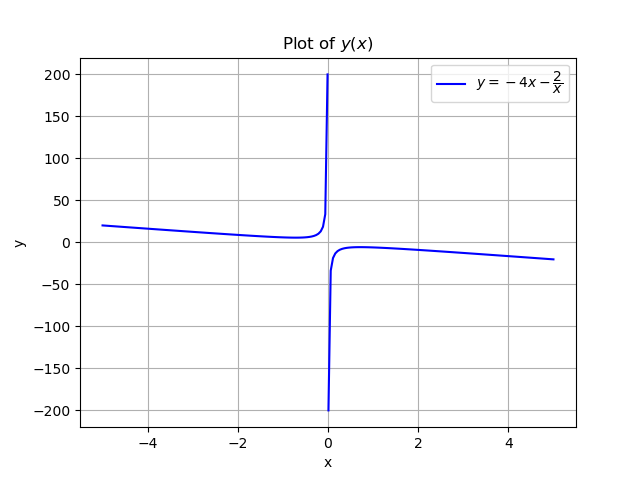
\includegraphics[width=\columnwidth]{figs/fig.png}
    \caption{Plot of $y(x)$ v/s $x$}
\end{figure}

\end{document}
